\section{The Machine Learning Models}
\subsection{Model selection}
In this analysis I have chosen to compare 4 different "types" of \ac{ML}-models, ordinary dense \acf{NN}, \acf{PNN},
ensemble and \acf{BDT}. The first three methods are all types of \ac{NN}. I have deliberately 
chosen to focus on \ac{NN} given that there is far more freedom in the design of the architecture
of a \ac{NN}, than compared to a XGboost. Additionally, this was motivated by the selfish reason
being that I found the networks more interesting to study and dissect. Therefore, most of the 
analysis, comparisons and discussion is focused on the networks, while XGBoost is included 
as a loose benchmark. 
\\
The choice of the three network architectures is motivated in wanting to compare a simple 
deep network, a network ensemble and a \ac{PNN}. I would assume that the optimal architecture
would be a network which combines elements from each, but for the purpose of discussion
and research I have chosen to keep them somewhat separate. 
\subsection{Creating custom layers}\label{subsec:CustomLayer}
The field of \ac{ML} is one of the most dynamic and fastest growing fields of research
today. This means, that regardless of the brave attempt made by voluntary contributors and
the people at Google\footnote{The developers of TensorFlow}, there will always be 
new and exciting \ac{ML} tools and algorithm, not yet implemented in their library. This was 
certainly the case in this thesis. For several of the non-dense layers I was forced
to dive into the world of \ac{ML} development and create my own implementation. 
\\
All ensemble methods described in section \ref{subsec:LWTA} (except for dropout), channel-out, 
\ac{SCO} and maxout, resemble a layer already implemented by Tensorflow. This layer is called MaxPooling1D
\footnote{For more information on MaxPoolind1D, the reader is referred to the documentation 
($\href{https://www.tensorflow.org/api_docs/python/tf/keras/layers/MaxPool1D}{https://www.tensorflow.org/api_docs/python/tf/keras/layers/MaxPool1D}$,
accessed 24.03.2023).}. But, to allow for experimentation I decided to not use MaxPooling1D, but instead 
implement my own custom layers. All custom layers were implemented by creating new functions inside 
TensorFlow's dense layer, which are called when the network makes a prediction. In the following sections 
I will describe the algorithms underlying the implementation of each layer.
\subsubsection*{Channel-out}
In algorithm \ref{alg:channel-out} I summarized the implementation of channel-out used in this analysis. For each 
input which is to be passed through a forward-pass, the function first passes it through the weights and biases 
as described in section \ref{subsec:FP}. This is true for all the other layers as well. In line 7 I reshape the input 
to add a dimension which creates the units. In line 10 I create a new variable, $Output$ by reducing each unit to the 
largest activated node. Further I set each node to 0 which is not equal to the largest activation. Finally, I reshape 
the output to the original shape and return the output.  
\begin{algorithm}
    \caption{The pseudocode for implementing the channel-out layer in TensorFlow}\label{alg:channel-out}
    \begin{algorithmic}[1]
    \State def \textbf{Channel-out}(Input): 
    \State \ \ \ \ $\%$ Pass input through weight kernel and adding bias terms.
    \State \ \ \ \ $Input \gets Input \times Weights$
    \State \ \ \ \ $Input \gets Input + Bias$
    \\
    \State \ \ \ \ $\%$ Reshape input into units
    \State \ \ \ \ $Input \gets \textbf{Reshape}(Input,(Nr\ Units,\ Size \ of \ Units))$
    \\
    \State \ \ \ \ $\%$ Reduce input to the largest activation in each unit.
    \State \ \ \ \ $Output \gets \textbf{Max}(Input)$
    \\
    \State \ \ \ \ $\%$ Set original activation where activation is largest and 0 where it's not.
    \State \ \ \ \ $Output \gets \textbf{Where}(Input == Output, Input,0)$
    \\
    \State \ \ \ \ $\%$ Reshape to original size.
    \State \ \ \ \ $Output \gets \textbf{Reshape}(Output,(Input's \ Original \ Shape))$
    \State \ \ \ \ $\textbf{return}\ Output$
    \end{algorithmic}
\end{algorithm}
\subsubsection*{SCO}
In section \ref{subsubsec:stochchannelout} I described how \ac{SCO} is an extension of channel-out. This is certainly
also the case for the algorithms explaining the implementation. In algorithm \ref{alg:SCO} I have described 
algorithm used in the implementation of \ac{SCO} in this analysis. Similar to channel-out, the algorithm begins by 
passing input through weights and biases. Then, contrary to channel-out the nodes of the input are shuffled. This 
is to ensure that when the input is reshaped (in line 10), the units are made differently for each pass through 
the function. Again the maximum activation is found to create a new variable, this time called $OutputShuffle$. 
In line 16 $InputShuflle$ and $OutputShuffle$ are compared such that where $InputShuflle$ is equal to the largest 
activation, the value is set to 1 and otherwise set to 0. $OutputShuffle$ is then unshuffled, and reshaped to the 
original shape. Finally, the input which has been passed through the weights and biases, is multiplied with 
$Output$ and returned.
\begin{algorithm}
    \caption{The pseudocode for implementing the SCO layer in TensorFlow}\label{alg:SCO}
    \begin{algorithmic}[1]
    \State def \textbf{SCO}(Input): 
    \State \ \ \ \ $\%$ Pass input through weight kernel and adding bias terms.
    \State \ \ \ \ $Input \gets Input \times Weights$
    \State \ \ \ \ $Input \gets Input + Bias$
    \\
    \State \ \ \ \ $\%$ Shuffle all the values
    \State \ \ \ \ $InputShuflle \gets \textbf{Shuffle}(Input)$
    \\
    \State \ \ \ \ $\%$ Reshape input into units
    \State \ \ \ \ $InputShuflle \gets \textbf{Reshape}(InputShuflle,(Nr\ Units,\ Size \ of \ Units))$
    \\
    \State \ \ \ \ $\%$ Reduce input to the largest activation in each unit.
    \State \ \ \ \ $OutputShuffle \gets \textbf{Max}(InputShuflle)$
    \\
    \State \ \ \ \ $\%$ Set 1 where activation is largest and 0 where not.
    \State \ \ \ \ $OutputShuffle \gets \textbf{Where}(InputShuflle == OutputShuffle, 1,0)$
    \\
    \State \ \ \ \ $\%$ Un-shuffle all the values
    \State \ \ \ \ $Output \gets \textbf{UnShuffle}(OutputShuffle)$
    \\
    \State \ \ \ \ $\%$ Reshape to original size.
    \State \ \ \ \ $Output \gets \textbf{Reshape}(Output,(Input's \ Original \ Shape))$
    \\
    \State \ \ \ \ $\%$ Multiply input with output to set all input that are not the largest, to zero.
    \State \ \ \ \ $NewOutput \gets Input \times Output$
    \\
    \State \ \ \ \ $\textbf{return}\ NewOutput$
    \end{algorithmic}
\end{algorithm}
\subsubsection*{Max-out}
In algorithm \ref{alg:maxout} I have summarized the algorithm behind the implementation of the maxout layer.
Off the three layers (channel-out, \ac{SCO} and maxout), maxout was the simplest to implement. After passing 
the input through the weights and biases and reshaped to form the units, the input is reduced to only include 
the largest activation in each layer. Finally, the output is reshaped to the original shape and returned.
\begin{algorithm}
    \caption{The pseudocode for implementing the maxout layer in TensorFlow}\label{alg:maxout}
    \begin{algorithmic}[1]
    \State def \textbf{MaxOut}(Input): 
    \State \ \ \ \ $\%$ Pass input through weight kernel and adding bias terms
    \State \ \ \ \ $Input \gets Input \times Weights$
    \State \ \ \ \ $Input \gets Input + Bias$
    \\
    \State \ \ \ \ $\%$ Reshape input into units
    \State \ \ \ \ $Input \gets \textbf{Reshape}(Input,(Nr\ Units,\ Size \ of \ Units))$
    \\
    \State \ \ \ \ $\%$ Reduce input to the largest activation in each unit
    \State \ \ \ \ $Output \gets \textbf{Max}(Input)$
    \\
    \State \ \ \ \ $\%$ Reshape to size equal the number of units.
    \State \ \ \ \ $Output \gets \textbf{Reshape}(Input,(Nr \ Units))$
    \State \ \ \ \ $\textbf{return}\ Input$
    \end{algorithmic}
\end{algorithm}
\subsection{Model Architecture}\label{subsec:arch}
When choosing a network architecture, there are several ways to proceed. One way is to apply a grid search.
A grid search is simply defining a grid of parameters to test, then running through all combinations and 
choosing the highest performer. With a sufficient amount of tests, a grid search should converge towards 
an optimal architecture. Grid search is very common and there exists a large range of very complex varieties \cite{GS}.
For my analysis I chose not to perform a grid search, for several reasons. The first being interpretability.
Understanding a \ac{NN} is already hard, allowing for complex and unique architectures would only add another layer
of mysticism. The second is the size of the data set. The larger the data set, the larger the amount of data 
would be needed to adequately perform tests for each combination of parameters. Not only is this time-consuming,
but trying to mediate this issue could lead to poor performance. The third and most important reason is that 
I wanted to experiment with the architectures. By manually tuning the parameters, I was able to achieve a far 
better understanding of the final architecture. 
\begin{figure}
    \makebox[0.9\linewidth][c]{%
    \centering
    \begin{subfigure}{1.1\textwidth}
        \centering
        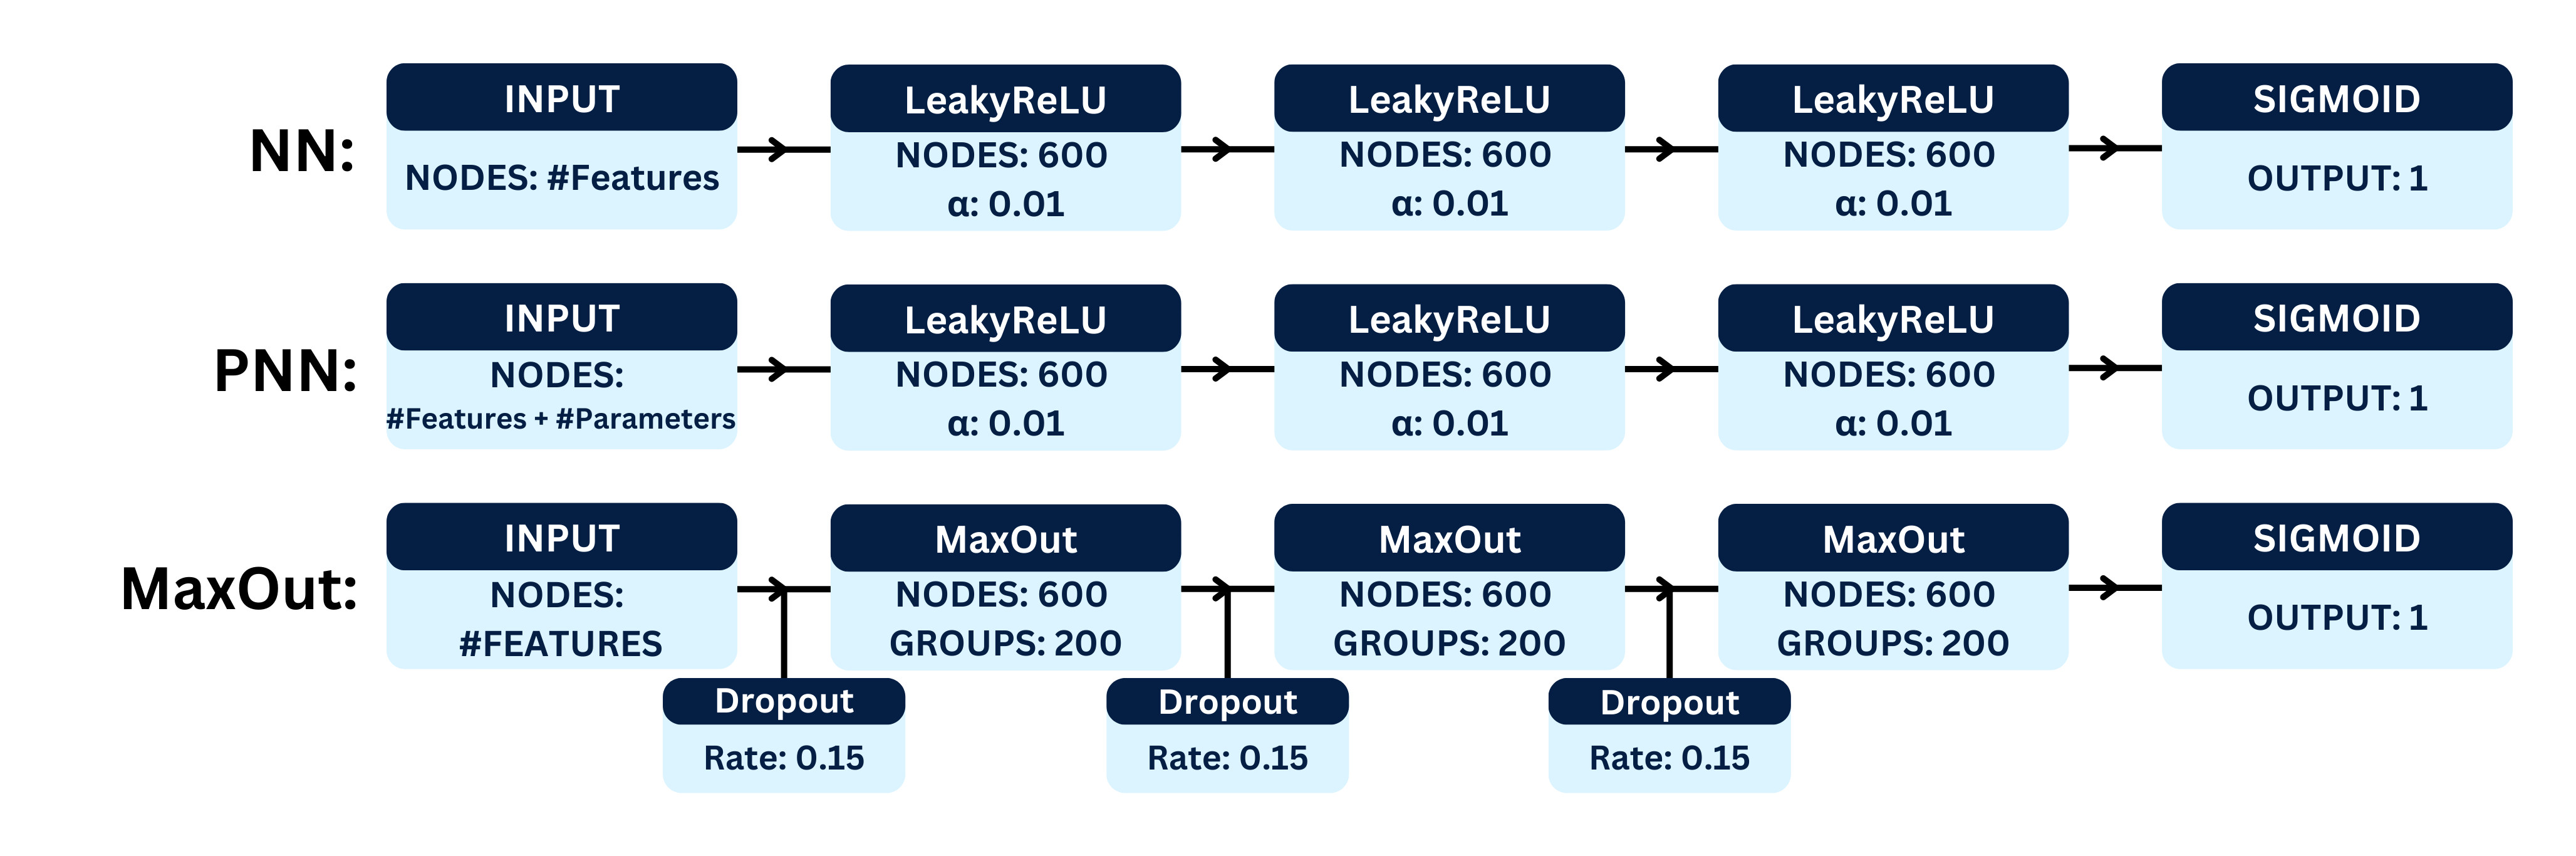
\includegraphics[width=\textwidth]{Figures/Illustrations/architecture.png}
    \end{subfigure}
    }
    \caption{A visual summary of the workflow and framework use for the 
    computational analysis. }
    \label{fig:arch}
\end{figure}
\subsection*{Dense Neural Network and PNN}\label{subsec:PNNArch}
The purpose of the simple dense \ac{NN}, is to compare the more complex networks to what is usually considered an ordinary dense \ac{NN}\footnote{Note 
that for the remaining part of this thesis, I will refer to this architecture as a 'dense \ac{NN}', 'ordinary dense \ac{NN}' and in some plots, just 
\ac{NN}}.
All layers are dense layers, meaning that all nodes in the previous layer are connected to the current layer, and likewise
the current layer is connected to the next. As is the default setting of the dense layer implemented in TensorFlow, the weights and biases are initialized 
using the so-called \emph{Glorot Uniform Initializer} (see the article by Glorot \cite{glorot_understanding_2010}, for more information). 
The general structure of the network is summarized in figure \ref{fig:arch}, with the network label \ac{NN}. The figure shows a dense \ac{NN} with 
three hidden layers, all with 600 nodes each. All hidden layers utilize the $LeakyReLU$ activation (see section \ref{subsec:activation})
with an $\alpha$ = 0.01. The architecture is designed to perform deep-training, and will train on a training set where all mass combinations 
are included\footnote{Contrary to training one network for each mass combination.}. 
\\
The \ac{PNN} architecture is like the name suggests, included to represent the model proposed by the article by Baldi et al. \cite{PNN}.
The architecture is illustrated in figure \ref{fig:arch}, with the label PNN. The figure shows a practically identical 
structure to the dense-\ac{NN}, with the only difference being in the input-layer. As was discussed in section \ref{subsec:PNN},
the \ac{PNN} includes the new physics signal free parameters\footnote{In our case, the masses of the \ac{BSM}-particles.} alongside the features
in the input layer.
\subsection*{MaxOut, Channel-Out and \ac{SCO}}
The ensemble methods are slightly more complex than both the dense \ac{NN} and \ac{PNN} in terms of architecture. To limit the complexity for comparison reasons
I choose to build an identical architecture for maxout, channel-Out and \ac{SCO}, with the only difference being which of the three layers is used.  
In figure \ref{fig:arch} I have illustrated the MaxOut architecture, with the label MaxOut. The figure shows a network with 6 hidden layers, 
3 MaxOut and 3 dropout. The network alternates between drop out and MaxOut, starting with dropout and finishing with MaxOut. The MaxOut layers 
have 600 nodes each which reduce down to the 200 nodes with the largest activation in their respective groups. Each dropout layer has a dropout 
rate of 0.15. Channel-out and \ac{SCO} have the same architecture to maxout, but replacing maxout with each of the two respectively. 

\subsection*{XGBoost}\label{subsec:XGBoost}
The main motivation to apply XGBoost is simply to benchmark my analysis, and therefore not a lot of effort has been put into the design of the 
architecture. As a consequence, the default parameters\footnote{See \href{https://xgboost.readthedocs.io/en/stable/parameter.html}
{https://xgboost.readthedocs.io/en/stable/parameter.html}
for a complete overview of default parameters.} of XGBoost have been used. The main parameters of the model are summarized as the following:
\begin{itemize}
    \item $\eta$ (learning-rate) = 0.3
    \item Max depth = 6
    \item Maximum number of trees = 100
\end{itemize}


